% Options for packages loaded elsewhere
\PassOptionsToPackage{unicode}{hyperref}
\PassOptionsToPackage{hyphens}{url}
\PassOptionsToPackage{dvipsnames,svgnames,x11names}{xcolor}
%
\documentclass[
]{article}

\usepackage{amsmath,amssymb}
\usepackage{iftex}
\ifPDFTeX
  \usepackage[T1]{fontenc}
  \usepackage[utf8]{inputenc}
  \usepackage{textcomp} % provide euro and other symbols
\else % if luatex or xetex
  \usepackage{unicode-math}
  \defaultfontfeatures{Scale=MatchLowercase}
  \defaultfontfeatures[\rmfamily]{Ligatures=TeX,Scale=1}
\fi
\usepackage{lmodern}
\ifPDFTeX\else  
    % xetex/luatex font selection
\fi
% Use upquote if available, for straight quotes in verbatim environments
\IfFileExists{upquote.sty}{\usepackage{upquote}}{}
\IfFileExists{microtype.sty}{% use microtype if available
  \usepackage[]{microtype}
  \UseMicrotypeSet[protrusion]{basicmath} % disable protrusion for tt fonts
}{}
\makeatletter
\@ifundefined{KOMAClassName}{% if non-KOMA class
  \IfFileExists{parskip.sty}{%
    \usepackage{parskip}
  }{% else
    \setlength{\parindent}{0pt}
    \setlength{\parskip}{6pt plus 2pt minus 1pt}}
}{% if KOMA class
  \KOMAoptions{parskip=half}}
\makeatother
\usepackage{xcolor}
\setlength{\emergencystretch}{3em} % prevent overfull lines
\setcounter{secnumdepth}{5}
% Make \paragraph and \subparagraph free-standing
\makeatletter
\ifx\paragraph\undefined\else
  \let\oldparagraph\paragraph
  \renewcommand{\paragraph}{
    \@ifstar
      \xxxParagraphStar
      \xxxParagraphNoStar
  }
  \newcommand{\xxxParagraphStar}[1]{\oldparagraph*{#1}\mbox{}}
  \newcommand{\xxxParagraphNoStar}[1]{\oldparagraph{#1}\mbox{}}
\fi
\ifx\subparagraph\undefined\else
  \let\oldsubparagraph\subparagraph
  \renewcommand{\subparagraph}{
    \@ifstar
      \xxxSubParagraphStar
      \xxxSubParagraphNoStar
  }
  \newcommand{\xxxSubParagraphStar}[1]{\oldsubparagraph*{#1}\mbox{}}
  \newcommand{\xxxSubParagraphNoStar}[1]{\oldsubparagraph{#1}\mbox{}}
\fi
\makeatother

\usepackage{color}
\usepackage{fancyvrb}
\newcommand{\VerbBar}{|}
\newcommand{\VERB}{\Verb[commandchars=\\\{\}]}
\DefineVerbatimEnvironment{Highlighting}{Verbatim}{commandchars=\\\{\}}
% Add ',fontsize=\small' for more characters per line
\usepackage{framed}
\definecolor{shadecolor}{RGB}{241,243,245}
\newenvironment{Shaded}{\begin{snugshade}}{\end{snugshade}}
\newcommand{\AlertTok}[1]{\textcolor[rgb]{0.68,0.00,0.00}{#1}}
\newcommand{\AnnotationTok}[1]{\textcolor[rgb]{0.37,0.37,0.37}{#1}}
\newcommand{\AttributeTok}[1]{\textcolor[rgb]{0.40,0.45,0.13}{#1}}
\newcommand{\BaseNTok}[1]{\textcolor[rgb]{0.68,0.00,0.00}{#1}}
\newcommand{\BuiltInTok}[1]{\textcolor[rgb]{0.00,0.23,0.31}{#1}}
\newcommand{\CharTok}[1]{\textcolor[rgb]{0.13,0.47,0.30}{#1}}
\newcommand{\CommentTok}[1]{\textcolor[rgb]{0.37,0.37,0.37}{#1}}
\newcommand{\CommentVarTok}[1]{\textcolor[rgb]{0.37,0.37,0.37}{\textit{#1}}}
\newcommand{\ConstantTok}[1]{\textcolor[rgb]{0.56,0.35,0.01}{#1}}
\newcommand{\ControlFlowTok}[1]{\textcolor[rgb]{0.00,0.23,0.31}{\textbf{#1}}}
\newcommand{\DataTypeTok}[1]{\textcolor[rgb]{0.68,0.00,0.00}{#1}}
\newcommand{\DecValTok}[1]{\textcolor[rgb]{0.68,0.00,0.00}{#1}}
\newcommand{\DocumentationTok}[1]{\textcolor[rgb]{0.37,0.37,0.37}{\textit{#1}}}
\newcommand{\ErrorTok}[1]{\textcolor[rgb]{0.68,0.00,0.00}{#1}}
\newcommand{\ExtensionTok}[1]{\textcolor[rgb]{0.00,0.23,0.31}{#1}}
\newcommand{\FloatTok}[1]{\textcolor[rgb]{0.68,0.00,0.00}{#1}}
\newcommand{\FunctionTok}[1]{\textcolor[rgb]{0.28,0.35,0.67}{#1}}
\newcommand{\ImportTok}[1]{\textcolor[rgb]{0.00,0.46,0.62}{#1}}
\newcommand{\InformationTok}[1]{\textcolor[rgb]{0.37,0.37,0.37}{#1}}
\newcommand{\KeywordTok}[1]{\textcolor[rgb]{0.00,0.23,0.31}{\textbf{#1}}}
\newcommand{\NormalTok}[1]{\textcolor[rgb]{0.00,0.23,0.31}{#1}}
\newcommand{\OperatorTok}[1]{\textcolor[rgb]{0.37,0.37,0.37}{#1}}
\newcommand{\OtherTok}[1]{\textcolor[rgb]{0.00,0.23,0.31}{#1}}
\newcommand{\PreprocessorTok}[1]{\textcolor[rgb]{0.68,0.00,0.00}{#1}}
\newcommand{\RegionMarkerTok}[1]{\textcolor[rgb]{0.00,0.23,0.31}{#1}}
\newcommand{\SpecialCharTok}[1]{\textcolor[rgb]{0.37,0.37,0.37}{#1}}
\newcommand{\SpecialStringTok}[1]{\textcolor[rgb]{0.13,0.47,0.30}{#1}}
\newcommand{\StringTok}[1]{\textcolor[rgb]{0.13,0.47,0.30}{#1}}
\newcommand{\VariableTok}[1]{\textcolor[rgb]{0.07,0.07,0.07}{#1}}
\newcommand{\VerbatimStringTok}[1]{\textcolor[rgb]{0.13,0.47,0.30}{#1}}
\newcommand{\WarningTok}[1]{\textcolor[rgb]{0.37,0.37,0.37}{\textit{#1}}}

\providecommand{\tightlist}{%
  \setlength{\itemsep}{0pt}\setlength{\parskip}{0pt}}\usepackage{longtable,booktabs,array}
\usepackage{calc} % for calculating minipage widths
% Correct order of tables after \paragraph or \subparagraph
\usepackage{etoolbox}
\makeatletter
\patchcmd\longtable{\par}{\if@noskipsec\mbox{}\fi\par}{}{}
\makeatother
% Allow footnotes in longtable head/foot
\IfFileExists{footnotehyper.sty}{\usepackage{footnotehyper}}{\usepackage{footnote}}
\makesavenoteenv{longtable}
\usepackage{graphicx}
\makeatletter
\newsavebox\pandoc@box
\newcommand*\pandocbounded[1]{% scales image to fit in text height/width
  \sbox\pandoc@box{#1}%
  \Gscale@div\@tempa{\textheight}{\dimexpr\ht\pandoc@box+\dp\pandoc@box\relax}%
  \Gscale@div\@tempb{\linewidth}{\wd\pandoc@box}%
  \ifdim\@tempb\p@<\@tempa\p@\let\@tempa\@tempb\fi% select the smaller of both
  \ifdim\@tempa\p@<\p@\scalebox{\@tempa}{\usebox\pandoc@box}%
  \else\usebox{\pandoc@box}%
  \fi%
}
% Set default figure placement to htbp
\def\fps@figure{htbp}
\makeatother

\usepackage{booktabs}
\usepackage{longtable}
\usepackage{array}
\usepackage{multirow}
\usepackage{wrapfig}
\usepackage{float}
\usepackage{colortbl}
\usepackage{pdflscape}
\usepackage{tabu}
\usepackage{threeparttable}
\usepackage{threeparttablex}
\usepackage[normalem]{ulem}
\usepackage{makecell}
\usepackage{xcolor}
\makeatletter
\@ifpackageloaded{caption}{}{\usepackage{caption}}
\AtBeginDocument{%
\ifdefined\contentsname
  \renewcommand*\contentsname{Indholdsfortegnelse}
\else
  \newcommand\contentsname{Indholdsfortegnelse}
\fi
\ifdefined\listfigurename
  \renewcommand*\listfigurename{Figuroversigt}
\else
  \newcommand\listfigurename{Figuroversigt}
\fi
\ifdefined\listtablename
  \renewcommand*\listtablename{Tabeloversigt}
\else
  \newcommand\listtablename{Tabeloversigt}
\fi
\ifdefined\figurename
  \renewcommand*\figurename{Figur}
\else
  \newcommand\figurename{Figur}
\fi
\ifdefined\tablename
  \renewcommand*\tablename{Tabel}
\else
  \newcommand\tablename{Tabel}
\fi
}
\@ifpackageloaded{float}{}{\usepackage{float}}
\floatstyle{ruled}
\@ifundefined{c@chapter}{\newfloat{codelisting}{h}{lop}}{\newfloat{codelisting}{h}{lop}[chapter]}
\floatname{codelisting}{Liste}
\newcommand*\listoflistings{\listof{codelisting}{Listeoversigt}}
\makeatother
\makeatletter
\makeatother
\makeatletter
\@ifpackageloaded{caption}{}{\usepackage{caption}}
\@ifpackageloaded{subcaption}{}{\usepackage{subcaption}}
\makeatother

\ifLuaTeX
\usepackage[bidi=basic]{babel}
\else
\usepackage[bidi=default]{babel}
\fi
\babelprovide[main,import]{danish}
% get rid of language-specific shorthands (see #6817):
\let\LanguageShortHands\languageshorthands
\def\languageshorthands#1{}
\usepackage{bookmark}

\IfFileExists{xurl.sty}{\usepackage{xurl}}{} % add URL line breaks if available
\urlstyle{same} % disable monospaced font for URLs
\hypersetup{
  pdftitle={Arbejdsløshed - Ugeeksamen i Forecasting},
  pdfauthor={Christine Hegelund; Jing Wei; Marcus Nielsen},
  pdflang={da},
  colorlinks=true,
  linkcolor={blue},
  filecolor={Maroon},
  citecolor={Blue},
  urlcolor={Blue},
  pdfcreator={LaTeX via pandoc}}


\title{Arbejdsløshed - Ugeeksamen i Forecasting}
\author{Christine Hegelund \and Jing Wei \and Marcus Nielsen}
\date{2025-06-13}

\begin{document}
\maketitle


\maketitle
\thispagestyle{empty}
\begin{center}
\large{Forecasting Eksamen} \\[3em]
\end{center}
\begin{center}
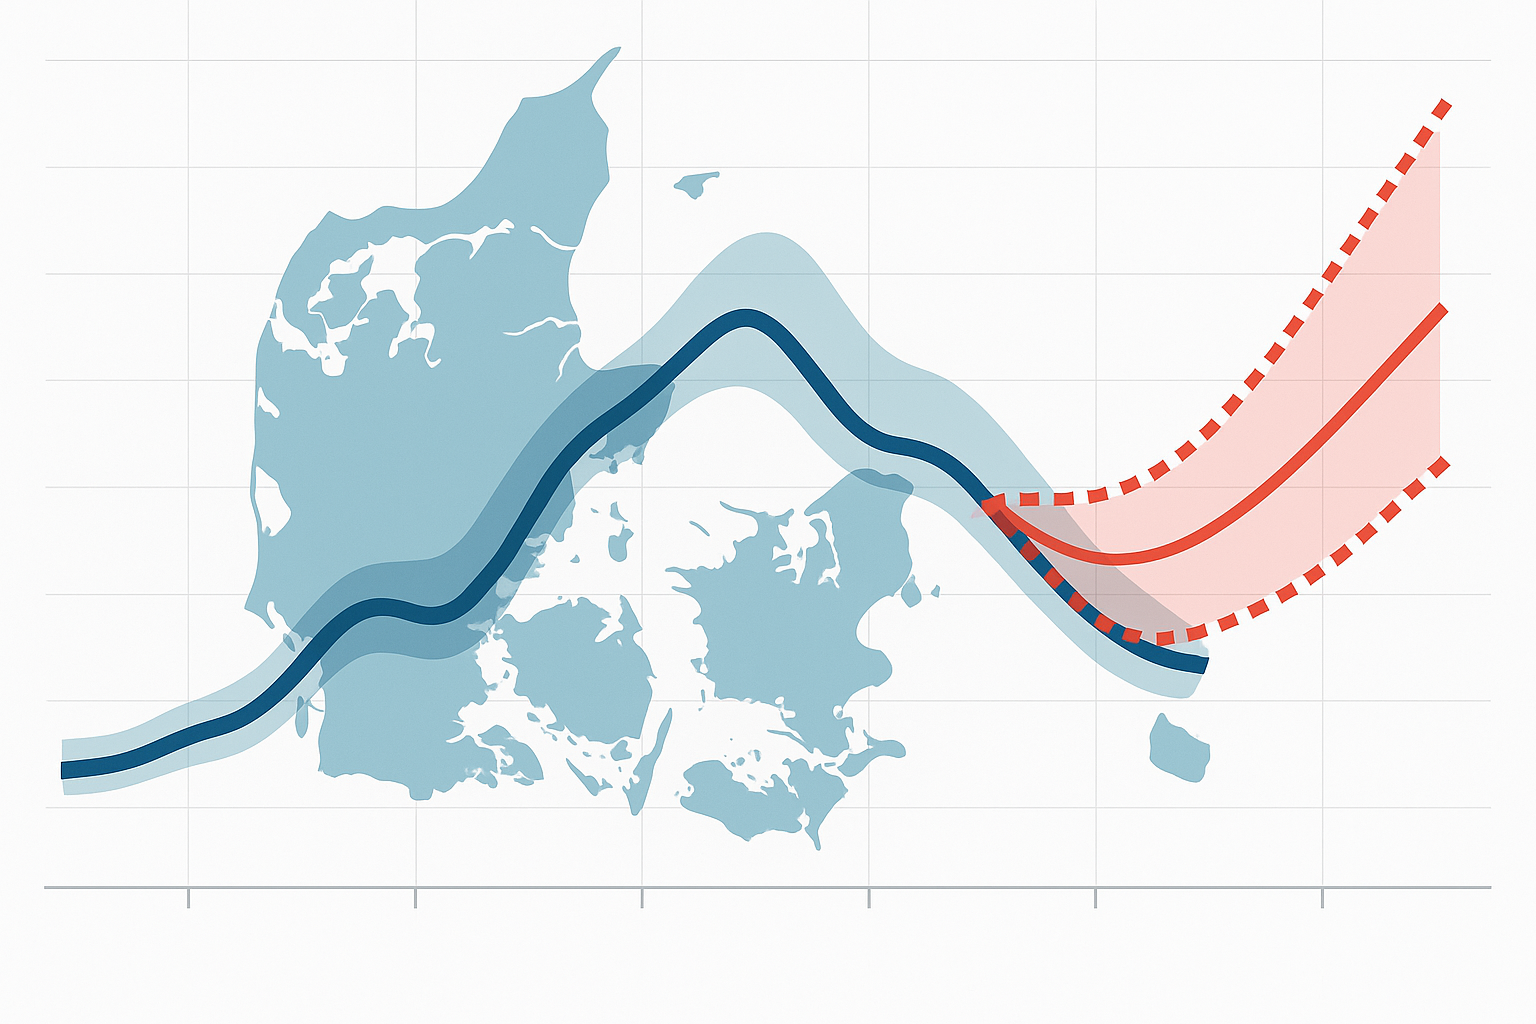
\includegraphics[width=0.9\textwidth]{fotos/forside.png} \\[2em]
\end{center}
\begin{center}
\fcolorbox{gray}{white}{
\parbox{0.8\textwidth}{
\centering
\textbf{Antal tegn (inkl. mellemrum): 97023}
}}
\end{center}
\begin{center}
\textbf{Vejledere:} \\
Bjarne Taulo Sørensen \\
\end{center}

\newpage

\tableofcontents

\section*{Tabel over figurer}\label{tabel-over-figurer}
\addcontentsline{toc}{section}{Tabel over figurer}

\thispagestyle{empty}

\newpage

\pagenumbering{arabic}
\setcounter{page}{1}
\tableofcontents
\newpage

\section{Introduktion}\label{introduktion}

Arbejdsløshedstal er en central indikator for et lands økonomiske
tilstand og udvikling. De påvirker både den enkelte borger og den
nationale økonomi og indgår som en væsentlig faktor i politiske og
økonomiske beslutningsprocesser. I takt med øget datatilgængelighed og
forbedrede statistiske værktøjer er det blevet muligt at analysere og
forudsige sådanne udviklingstræk med større præcision.

Denne opgave undersøger udviklingen i arbejdsløsheden i Danmark i
perioden 2007 til 2019 -- opdelt på køn og region. Datagrundlaget består
af ti tidsserier, én for hver kombination af fem regioner og to køn. Det
giver mulighed for at analysere både regionale forskelle og
kønsspecifikke mønstre i arbejdsløsheden.

Med udgangspunkt i klassiske tidsseriemodeller, ARIMA, ETS og en simpel
benchmarkmodel (Seasonal Naive), undersøges, hvordan arbejdsløsheden har
udviklet sig, og hvordan den kan fremskrives. Undervejs vurderes
modellernes egnethed med fokus på præcision og residualstruktur, og der
anvendes teknikker som STL-dekomposition og transformation af data.
Målet er ikke blot at forudsige udviklingen i 2020, men også at vurdere,
hvor godt klassiske modeller formår at håndtere forskellene mellem
regioner og køn.

\section{Problemformulering}\label{problemformulering}

Hvordan kan klassiske tidsseriemodeller anvendes til at analysere og
forudsige udviklingen i arbejdsløsheden i Danmark, fordelt på region og
køn?

For at besvare dette spørgsmål undersøges følgende delspørgsmål:

\begin{enumerate}
\def\labelenumi{\arabic{enumi}.}
\item
  Hvordan varierer arbejdsløshedens udvikling og sæsonmønstre på tværs
  af regioner og køn, og hvordan kan disse identificeres gennem
  eksplorativ dataanalyse og dekomposition?
\item
  Hvordan performer modellerne ARIMA, ETS og Seasonal Naive i forhold
  til hinanden, når det gælder præcision, residualstruktur og
  prognoseegenskaber?
\item
  Hvilke modeller er bedst egnede til at fremskrive
  arbejdsløshedstallene for 2020, og hvordan varierer usikkerheden på
  tværs af serier?
\end{enumerate}

\subsection{Afgrænsning}\label{afgruxe6nsning}

Analysen bygger udelukkende på de udleverede arbejdsløshedsdata for
perioden januar 2007 til december 2019 og inddrager ikke eksterne
forklarende faktorer som COVID-19, konjunkturudsving eller politiske
tiltag. Formålet er ikke at forklare årsager til ledighed, men at
undersøge, hvordan klassiske forecasting-modeller kan anvendes metodisk
og reproducerbart. Fokus ligger på statistisk modellering og
sammenligning af modelpræcision -- ikke på strategiske eller politiske
anbefalinger.

\subsubsection{Anvendelse af
AI-værktøj}\label{anvendelse-af-ai-vuxe6rktuxf8j}

ChatGPT (GPT-4o) er anvendt som støtteværktøj i forbindelse med
idéudvikling, sproglig formulering og udformning af enkelte kodestumper.
Værktøjet er kun brugt til tekniske og sproglige formål -- al analyse,
fortolkning og konklusion er udarbejdet selvstændigt af gruppens
medlemmer.

\subsection{Definitioner/forkortelser}\label{definitionerforkortelser}

Nedenfor er en oversigt over centrale begreber og forkortelser, som
anvendes i opgaven:

\begin{itemize}
\tightlist
\item
  \textbf{ARIMA}: AutoRegressive Integrated Moving Average
\item
  \textbf{ETS}: Exponential Smoothing State Space Model
\item
  \textbf{SNAÏVE}: Seasonal Naive
\item
  \textbf{RMSE}: Root Mean Squared Error
\item
  \textbf{MAPE}: Mean Absolute Percentage Error
\item
  \textbf{STL}: Seasonal-Trend decomposition using Loess
\item
  \textbf{CV}: Cross-validation
\end{itemize}

\subsection{Struktur}\label{struktur}

Opgaven er opbygget i fem hovedfaser, som følger en klassisk tilgang til
analyse af tidsserier. Først gennemføres en eksplorativ dataanalyse
(EDA), hvor dataserierne visualiseres og undersøges for tendenser,
sæsonmønstre og variation. Dette sker med grafer, deskriptive
statistikker og STL-dekomposition, og data transformeres efter behov.
Derefter estimeres tre modeltyper -- ARIMA, ETS og Seasonal Naive -- for
hver serie. Modellerne valideres med krydsvalidering, residualanalyse og
forecast-metrikker, før de anvendes til at fremskrive arbejdsløsheden
for 2020 med tilhørende usikkerhed. Til sidst sammenlignes modeller og
ledighedsniveauer på tværs af regioner og køn, og der konkluderes på den
overordnede problemstilling.

\section{Data og forberedelse}\label{data-og-forberedelse}

Analysen bygger på månedlige arbejdsløshedstal fra Danmark i perioden
januar 2007 til december 2019. Data er opdelt efter køn og region,
hvilket giver ti separate tidsserier. Datasættet er udleveret i et
forbehandlet tsibble-format med tydeligt definerede indeks- og
nøglevariabler, og nedenfor indlæses datasættet:

\begin{verbatim}
# A tsibble: 6 x 4 [1M]
# Key:       kon, region [1]
  kon     region             yearmonth svalue
  <fct>   <fct>                  <mth>  <dbl>
1 Kvinder Region Hovedstaden  2007 Jan   2.26
2 Kvinder Region Hovedstaden  2007 Feb   2.19
3 Kvinder Region Hovedstaden  2007 Mar   2.09
4 Kvinder Region Hovedstaden  2007 Apr   1.97
5 Kvinder Region Hovedstaden  2007 May   1.99
6 Kvinder Region Hovedstaden  2007 Jun   1.93
\end{verbatim}

\section{Eksplorativ dataanalyse
(EDA)}\label{eksplorativ-dataanalyse-eda}

Formålet med dette afsnit er at skabe et overblik over datasættets
struktur forud for modelleringen. Ved hjælp af visualiseringer,
deskriptive statistikker og STL-dekomposition undersøges
arbejdsløshedens udvikling på tværs af regioner og køn i perioden
2007--2019. Analysen afdækker overordnede tendenser, sæsonmønstre og
forskelle i niveau og variation. For at sikre god modellering vurderes
behovet for datatransformation, og tidsserierne dekomponeres i trend,
sæson og residualer. Resultaterne danner det metodiske fundament for det
videre modelarbejde.

\subsection{Visualisering af udvikling og
mønstre}\label{visualisering-af-udvikling-og-muxf8nstre}

I dette afsnit undersøges, hvordan arbejdsløsheden har udviklet sig over
tid -- med fokus på tendenser, sæsonvariationer og forskelle mellem
regioner og køn. Formålet er at identificere mønstre, som kan guide valg
af modeller i den videre analyse.

\subsubsection{Udvikling over tid}\label{udvikling-over-tid}

I de følgende figurer undersøges udviklingen i arbejdsløsheden over tid.
Til at begynde med anvendes den oprindelige skala for at give et
lettilgængeligt overblik (Figur 1 og 2). Fra Figur 3 og frem benyttes en
log-transformation for at stabilisere variationen i serierne, især
blandt mænd, og for at sikre sammenlignelighed i videre modellering og
forecast.

\textbf{Figur 1: Udvikling i kvinders arbejdsløshed pr. region}

\pandocbounded{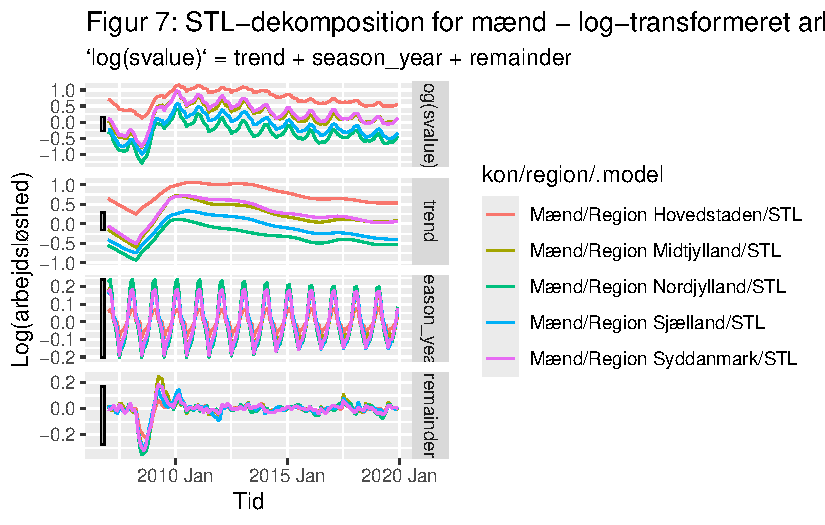
\includegraphics[keepaspectratio]{130625_Forecasting_files/figure-pdf/unnamed-chunk-2-1.pdf}}

Figuren viser den månedlige arbejdsløshed blandt kvinder i de fem danske
regioner fra 2007 til 2019. Der fremgår et tydeligt sæsonmønster med
højere ledighed i vintermånederne og lavere i sommerperioden. Niveauet
varierer regionalt, hvor Region Hovedstaden typisk ligger højest og
Nordjylland lavest. Samlet ses en faldende tendens efter finanskrisen.

\textbf{Figur 2: Udvikling i mænds arbejdsløshed pr. region}

\pandocbounded{\includegraphics[keepaspectratio]{130625_Forecasting_files/figure-pdf/unnamed-chunk-3-1.pdf}}

Sammenlignet med kvinder ses større udsving og et generelt højere niveau
i mænds arbejdsløshed. Sæsonmønstrene er mere markante, og variationen
mellem regionerne er tydeligere -- især i Region Syddanmark og
Midtjylland, hvor krisen i 2008-2009 medfører et kraftigt midlertidigt
løft i ledigheden.

\textbf{Figur 3: Udvikling i arbejdsløshed hos pr. region og køn
(log-skala)}

\pandocbounded{\includegraphics[keepaspectratio]{130625_Forecasting_files/figure-pdf/unnamed-chunk-4-1.pdf}}

Figur 3 viser, hvordan arbejdsløsheden har udviklet sig for mænd og
kvinder i de fem danske regioner -- både på original og
log-transformeret skala.\\
De stiplede linjer repræsenterer de oprindelige værdier, mens de fuldt
optrukne linjer viser samme udvikling på log-skala. Log-transformationen
gør det nemmere at få øje på mønstre og forskelle, især i serier med
store udsving eller høj varians. Hvor den oprindelige skala fremhæver de
absolutte niveauer, giver log-skalaen et mere balanceret overblik over
den relative udvikling. Den log-transformerede fremstilling danner
derfor grundlag for den videre analyse.

\subsubsection{Sæsonmønstre}\label{suxe6sonmuxf8nstre}

Med log-transformerede data som fundament undersøges nu sæsonmønstrene i
arbejdsløsheden nærmere. Gennem sæsonplots og subserieplots vurderes,
hvordan arbejdsløsheden typisk varierer over året -- og hvordan dette
adskiller sig mellem mænd og kvinder samt på tværs af regioner.

\textbf{Figur 4: Sæsonmønster for mænd pr. region}

\pandocbounded{\includegraphics[keepaspectratio]{130625_Forecasting_files/figure-pdf/unnamed-chunk-5-1.pdf}}

Figur 4 viser sæsonmønstre i mænds arbejdsløshed fordelt på regioner.
Hver farvet linje repræsenterer et år, og linjernes forløb illustrerer,
hvordan arbejdsløsheden typisk er højest i årets begyndelse
(januar--marts) og lavest i sommermånederne (juni--august). Mønsteret er
relativt konsistent på tværs af år og regioner, hvilket understøtter
tilstedeværelsen af en stabil sæsonkomponent i mænds ledighed. De
højeste niveauer ses i Region Hovedstaden, mens Region Sjælland og
Region Nordjylland ligger lavere. Bemærk især det markante fald fra
marts til juni, som gentager sig på tværs af årstal.

\textbf{Figur 5: Sæsonmønster for kvinder pr. region}

\pandocbounded{\includegraphics[keepaspectratio]{130625_Forecasting_files/figure-pdf/unnamed-chunk-6-1.pdf}}

Sammenlignet med mænd er sæsonudsvingene blandt kvinder mindre udtalte,
og udviklingen fremstår mere jævn og stabil på tværs af årene.
Niveauforskellene mellem regionerne er bevaret, men udsvingene over
måneder er mere afdæmpede. Det indikerer en lavere volatilitet i
kvinders arbejdsløshed og en mere ensartet sæsonprofil.

\textbf{Figur 6: Subserieplot for mænd pr. måned og region}

\pandocbounded{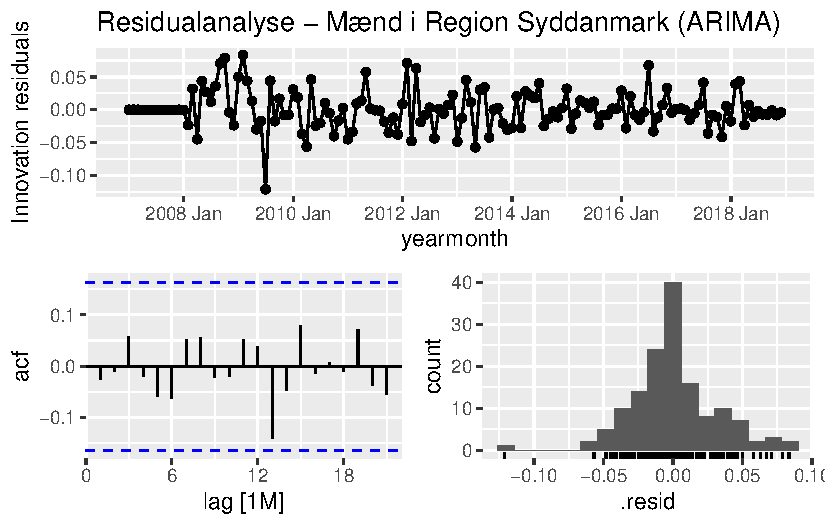
\includegraphics[keepaspectratio]{130625_Forecasting_files/figure-pdf/unnamed-chunk-7-1.pdf}}

Figur 6 viser udviklingen i mænds arbejdsløshed fordelt på måneder og
regioner, hvor hver facetteret celle repræsenterer en måned. Den sorte
linje viser udviklingen over tid, mens den blå streg repræsenterer
gennemsnittet. Det ses, at arbejdsløsheden konsekvent topper i årets
første måneder og falder hen over sommeren. Desuden er udsvingene mellem
år særligt store i vinterhalvåret, hvilket understreger en høj
sæsonafhængighed og volatilitet i mænds ledighedsniveau. Mønstret er
gennemgående i alle regioner, om end niveauet varierer.

\textbf{Figur 7: Subserieplot for kvinder pr. måned og region}

\pandocbounded{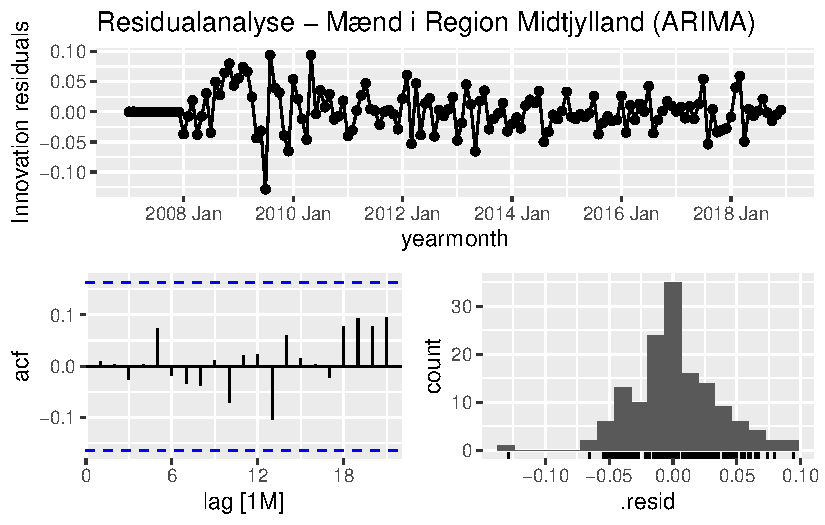
\includegraphics[keepaspectratio]{130625_Forecasting_files/figure-pdf/unnamed-chunk-8-1.pdf}}

Sammenlignet med mænd viser kvinder tilsvarende sæsonmønstre med højere
ledighed i årets begyndelse og lavere i sommermånederne. Udsvingene er
dog mindre markante, og variationen mellem år er mindre tydelig.
Mønstret fremstår mere stabilt og jævnt fordelt på tværs af regioner,
hvilket tyder på lavere volatilitet i kvindernes arbejdsløshed.

Udover sæsonmæssige udsving varierer arbejdsløsheden betydeligt på tværs
af både geografi og køn. Dette undersøges nærmere i de følgende
visualiseringer.

\subsubsection{Regionale og kønsmæssige
forskelle}\label{regionale-og-kuxf8nsmuxe6ssige-forskelle}

I dette afsnit rettes fokus mod samspillet mellem køn og region. Der
undersøges, hvordan forskelle i arbejdsløshedsniveau og -mønstre
varierer både mellem regioner og mellem mænd og kvinder.
Visualiseringerne præsenteres i forskellige facetteringer for at
fremhæve de vigtigste forskelle.

\textbf{Figur 8: Arbejdsløshed fordelt på regioner -- opdelt efter køn}

\pandocbounded{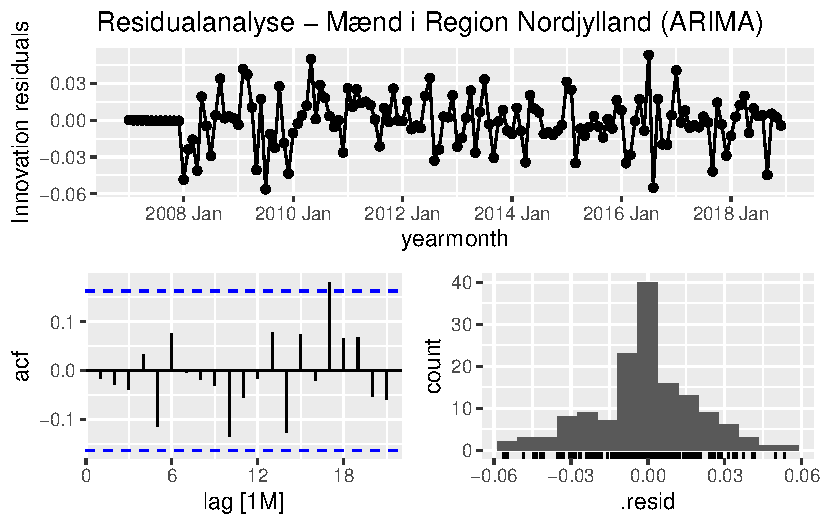
\includegraphics[keepaspectratio]{130625_Forecasting_files/figure-pdf/unnamed-chunk-9-1.pdf}}

Figur 8 viser den log-transformerede udvikling i arbejdsløsheden blandt
mænd og kvinder, fordelt på regioner. Hver farve repræsenterer en
region, og mænd og kvinder vises i hver sin fane, så det er lettere at
sammenligne på tværs. Log-skalaen gør forskellene mellem regionerne mere
overskuelige og dæmper de største udsving. Niveauet er stadig højest i
Region Hovedstaden og lavest i Nordjylland. Der er tydelige
sæsonbevægelser, særligt blandt mænd, hvor udsvingene fortsat er størst.
For kvinder fremstår udviklingen mere jævn.

\textbf{Figur 9: Arbejdsløshed fordelt på køn -- opdelt efter region}

\pandocbounded{\includegraphics[keepaspectratio]{130625_Forecasting_files/figure-pdf/unnamed-chunk-10-1.pdf}}

Hvor Figur 8 fokuserede på at sammenligne regioner inden for hvert køn,
giver Figur 9 et omvendt perspektiv: her sammenlignes køn i hver af de
fem danske regioner. Mænd har generelt højere arbejdsløshed og mere
markante udsving end kvinder -- særligt i perioden omkring finanskrisen.
Forskellene mellem kønnene er forholdsvis stabile på tværs af regioner,
men mønstret bekræfter, at mænds ledighed både topper højere og varierer
mere over tid. Kvindernes ledighed er lavere og udvikler sig mere
glidende. Figuren understøtter dermed beslutningen om at analysere
serierne individuelt. Samlet set viser figurerne, at arbejdsløsheden
varierer tydeligt mellem både regioner og køn, hvilket bekræfter
relevansen af at behandle hver tidsserie separat i den videre analyse.
Som næste skridt suppleres med deskriptive statistikker, der opsummerer
forskelle i niveau og udsving.

\subsection{Deskriptive statistikker}\label{deskriptive-statistikker}

For at supplere graferne anvendes deskriptive statistikker som
gennemsnit, spredning, minimum og maksimum. De opsummerer niveau og
variation i arbejdsløsheden pr. region og køn (Hyndman \&
Athanasopoulos, 2021). Statistikkerne giver et hurtigt overblik over
forskelle mellem grupper og hjælper med at identificere serier med høj
volatilitet. Det bidrager til at vurdere, hvor der kan være behov for
særlig opmærksomhed i den videre modellering.

\begin{longtable}[t]{llrrrr}
\caption{Deskriptiv statistik per region og køn}\\
\toprule
\cellcolor[HTML]{f0f0f0}{\textbf{region}} & \cellcolor[HTML]{f0f0f0}{\textbf{kon}} & \cellcolor[HTML]{f0f0f0}{\textbf{Gennemsnit}} & \cellcolor[HTML]{f0f0f0}{\textbf{Standardafvigelse}} & \cellcolor[HTML]{f0f0f0}{\textbf{Minimum}} & \cellcolor[HTML]{f0f0f0}{\textbf{Maksimum}}\\
\midrule
Region Hovedstaden & Kvinder & 2.07 & 0.36 & 1.13 & 2.67\\
Region Hovedstaden & Mænd & 2.17 & 0.52 & 1.13 & 3.18\\
Region Midtjylland & Kvinder & 1.27 & 0.25 & 0.58 & 1.72\\
Region Midtjylland & Mænd & 1.29 & 0.44 & 0.45 & 2.62\\
Region Nordjylland & Kvinder & 0.67 & 0.10 & 0.38 & 1.09\\
\addlinespace
Region Nordjylland & Mænd & 0.74 & 0.23 & 0.28 & 1.50\\
Region Sjælland & Kvinder & 0.86 & 0.17 & 0.45 & 1.20\\
Region Sjælland & Mænd & 0.92 & 0.30 & 0.37 & 1.78\\
Region Syddanmark & Kvinder & 1.24 & 0.26 & 0.60 & 1.76\\
Region Syddanmark & Mænd & 1.37 & 0.47 & 0.47 & 2.65\\
\bottomrule
\end{longtable}

Tabel 1 opsummerer arbejdsløsheden på tværs af regioner og køn.
Gennemsnittet viser det generelle niveau, mens standardafvigelsen giver
et mål for variation over tid. Mænd har generelt højere gennemsnit og
større udsving end kvinder, særligt i Region Hovedstaden og Syddanmark.
Omvendt ses lavere og mere stabile niveauer i Nordjylland, især blandt
kvinder. Minimums- og maksimumværdier understøtter indtrykket af høj
volatilitet i visse serier -- hvilket kan få betydning for modelvalget i
næste fase.

\subsection{STL-dekomposition}\label{stl-dekomposition}

For at opnå en bedre forståelse af de strukturelle komponenter i
arbejdsløshedsserierne anvendes STL-dekomposition (Seasonal-Trend
decomposition using Loess). Metoden adskiller tidsserier i tre
komponenter: trend, sæson og remainder (Hyndman \& Athanasopoulos,
2021). Det giver indblik i, hvor meget af variationen der kan forklares
af langsigtede bevægelser, gentagne sæsonmønstre eller kortsigtede,
uregelmæssige udsving.

Da særligt mændenes serier udviser høje niveauer og større variation, er
alle serier log-transformeret forud for dekompositionen. Denne
transformation stabiliserer variansen og gør det lettere at sammenligne
komponenterne på tværs af regioner og køn.

STL anvendes her på de log-transformerede serier for henholdsvis kvinder
og mænd i hver region. Resultaterne præsenteres i figur 10 og 11.

\textbf{Figur 10: STL-dekomposition for kvinder -- log-transformeret
arbejdsløshed pr. region}

\pandocbounded{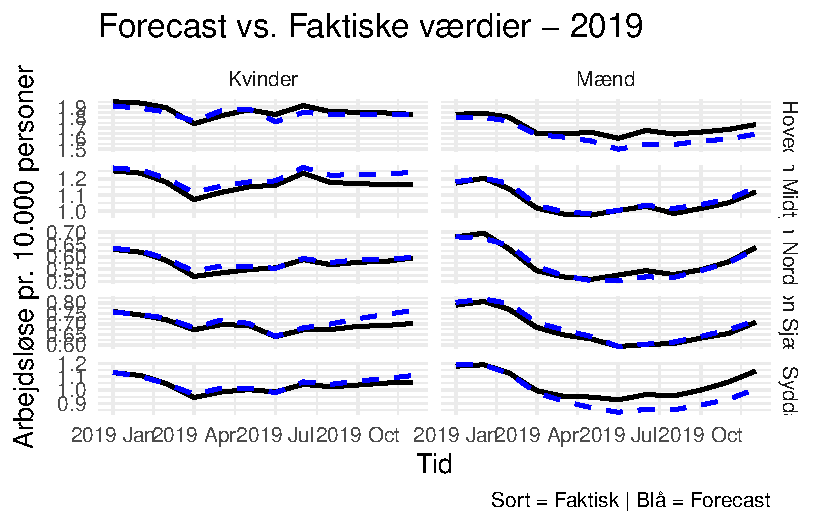
\includegraphics[keepaspectratio]{130625_Forecasting_files/figure-pdf/unnamed-chunk-11-1.pdf}}

Figur 10 viser STL-dekompositionen for kvinder i de fem danske regioner.
Der ses tydelige sæsonmønstre med tilbagevendende lavpunkter i
sommermånederne og højere ledighed i vinterhalvåret. Trends varierer
mellem regionerne: Region Hovedstaden udviser generelt højere ledighed,
mens Nordjylland og Sjælland ligger lavere. Residualerne ligger stabilt
omkring nul, hvilket indikerer, at modellen formår at fange de
dominerende strukturer i data.

\textbf{Figur 11: STL-dekomposition for mænd -- log-transformeret
arbejdsløshed pr. region}

\pandocbounded{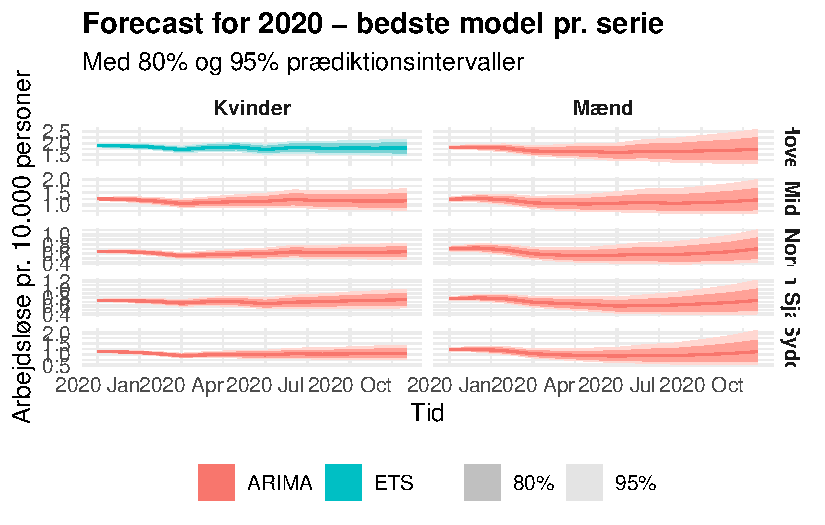
\includegraphics[keepaspectratio]{130625_Forecasting_files/figure-pdf/unnamed-chunk-12-1.pdf}}

Figur 11 viser tilsvarende dekomposition for mænd. Her ses en
tilsvarende stærk sæsonkomponent, men med mere markante udsving og
højere ledighedsniveauer -- især efter finanskrisen. Trends følger samme
overordnede forløb som for kvinder, men afvigelserne er større. Dette
bekræfter tidligere observationer om højere volatilitet i mænds
ledighed. Residualkomponenten er mere varierende, hvilket kan indikere,
at nogle udsving ikke fanges fuldt ud af modellen.

Disse observationer fra STL-dekompositionen bekræfter, at både trend og
sæsonmønstre varierer betydeligt på tværs af serierne. Det understreger
behovet for modeller, der kan tilpasses hver series struktur, hvilket
vil blive præsenteret i det følgende afsnit.

\section{Modelvalg}\label{modelvalg}

I dette afsnit estimeres og sammenlignes tre klassiske modeltyper,
ARIMA, ETS og benchmarkmodellen SNaive, for hver tidsserie (region ×
køn). Hver modeltype har forskellige antagelser og fordele og kan fange
forskellige karakteristika i data, såsom trend, sæson og
autokorrelation. Modelvalget foretages automatisk for hver serie via
fable-pakken, og resultaterne anvendes i den efterfølgende validering og
forecast.

\subsection{Valgte modeltyper}\label{valgte-modeltyper}

\textbf{ARIMA (AutoRegressive Integrated Moving Average)}\\
ARIMA-modeller anvendes til at modellere tidsserier med autokorrelation
og ikke-stationaritet. De kombinerer autoregressive (AR) led, differens
(I) for at opnå stationaritet, og glidende gennemsnit (MA) led til at
modellere fejl. Ved at inkludere sæsonkomponenter (SARIMA) kan modellen
håndtere årligt gentagende mønstre. ARIMA er særligt velegnet til serier
med langsigtede trends og strukturelle skift, hvor tidligere værdier har
stor indflydelse på den nuværende tilstand (jf. Hyndman \&
Athanasopoulos, kap. 9).

\textbf{ETS (Exponential Smoothing State Space Model)}\\
ETS-modeller benytter eksponentiel glatning til at vægte nyere
observationer højere og beskriver tidsserier ud fra tre elementer: fejl,
trend og sæson. Hver komponent kan være additiv eller multiplicativ
afhængigt af dataens karakter. ETS egner sig godt til serier med
tydelige strukturer og sæsonrytmer, især når der ikke er behov for at
modellere autokorrelation direkte (jf. kap. 8).

\textbf{SNAÏVE (Seasonal Naive)}\\
SNaive er en enkel benchmarkmodel, der baserer hvert forecast på den
tilsvarende værdi fra samme sæson i den foregående periode. Modellen
fanger sæsonmønstre, men tager ikke højde for trend eller afhængighed i
data. Den anvendes til at vurdere, om mere komplekse modeller giver en
mærkbart bedre forecast-præcision (jf. kap. 3 og 8).

\subsection{Modellering i praksis}\label{modellering-i-praksis}

Ved hjælp af fable-pakken estimeres de tre modeller automatisk for hver
af de ti tidsserier på baggrund af data fra 2007 til 2019. Herefter
genereres forecasts for 2020 med tilhørende prædiktionsintervaller.
Prognoserne visualiseres, så man kan sammenligne modellernes adfærd på
tværs af regioner og køn.

\begin{longtable}[t]{llll}
\caption{Automatisk valgte modelstrukturer for hver serie (region × køn)}\\
\toprule
\cellcolor[HTML]{f0f0f0}{\textbf{kon}} & \cellcolor[HTML]{f0f0f0}{\textbf{region}} & \cellcolor[HTML]{f0f0f0}{\textbf{.model}} & \cellcolor[HTML]{f0f0f0}{\textbf{AICc}}\\
\midrule
Kvinder & Region Hovedstaden & ARIMA & -519.59277\\
Kvinder & Region Hovedstaden & ETS & -106.04957\\
Kvinder & Region Hovedstaden & SNaive & NA\\
Kvinder & Region Midtjylland & ARIMA & -559.62392\\
Kvinder & Region Midtjylland & ETS & -186.73947\\
\addlinespace
Kvinder & Region Midtjylland & SNaive & NA\\
Kvinder & Region Nordjylland & ARIMA & -794.48456\\
Kvinder & Region Nordjylland & ETS & -420.44010\\
Kvinder & Region Nordjylland & SNaive & NA\\
Kvinder & Region Sjælland & ARIMA & -714.46022\\
\addlinespace
Kvinder & Region Sjælland & ETS & -355.53652\\
Kvinder & Region Sjælland & SNaive & NA\\
Kvinder & Region Syddanmark & ARIMA & -615.90506\\
Kvinder & Region Syddanmark & ETS & -194.25088\\
Kvinder & Region Syddanmark & SNaive & NA\\
\addlinespace
Mænd & Region Hovedstaden & ARIMA & -451.76084\\
Mænd & Region Hovedstaden & ETS & -94.42293\\
Mænd & Region Hovedstaden & SNaive & NA\\
Mænd & Region Midtjylland & ARIMA & -365.22171\\
Mænd & Region Midtjylland & ETS & 24.67626\\
\addlinespace
Mænd & Region Midtjylland & SNaive & NA\\
Mænd & Region Nordjylland & ARIMA & -536.74821\\
Mænd & Region Nordjylland & ETS & -202.87509\\
Mænd & Region Nordjylland & SNaive & NA\\
Mænd & Region Sjælland & ARIMA & -524.52351\\
\addlinespace
Mænd & Region Sjælland & ETS & -271.66140\\
Mænd & Region Sjælland & SNaive & NA\\
Mænd & Region Syddanmark & ARIMA & -387.29279\\
Mænd & Region Syddanmark & ETS & -55.07382\\
Mænd & Region Syddanmark & SNaive & NA\\
\bottomrule
\end{longtable}

Modelvalget er gennemført for hver enkelt tidsserie ved automatisk
estimering af ARIMA-, ETS- og SNaive-modeller med fable-pakken.
Udvælgelsen er sket på baggrund af AICc, som sikrer en afbalanceret
vurdering af modelkompleksitet og tilpasningsevne -- særligt vigtigt for
relativt korte tidsserier. Resultaterne i Tabel 2 viser, at modellerne
varierer betydeligt på tværs af køn og regioner, hvilket understreger
nødvendigheden af en differentieret strategi, hvor hver tidsserie
behandles individuelt.

SNaive-modellen er anvendt som benchmark og danner referencepunkt for
den efterfølgende evaluering. Den egentlige vurdering af modellernes
forecast-præcision foretages først i næste afsnit, hvor modellerne
sammenlignes på baggrund af tidsserie-krydsvalidering og metrikker som
RMSE og MAPE.

\section{Modelvalidering}\label{modelvalidering}

For at opnå en robust vurdering kombineres testsplit og time series
cross-validation. Testsplittet simulerer en realistisk
forecast-situation, mens cross-validation måler præcisionen over flere
tidspunkter og reducerer risikoen for tilfældige variationer.

\subsection{Trænings- og testsplit}\label{truxe6nings--og-testsplit}

Datasættet opdeles i en træningsperiode (2007--2018) og en testperiode
(2019). Modellerne estimeres på træningsdata og genererer forecasts for
teståret. Præcisionen vurderes ved sammenligning med de faktiske
observationer fra 2019.

\subsection{Evalueringsmetrikker: RMSE og
MAPE}\label{evalueringsmetrikker-rmse-og-mape}

For at vurdere, hvor godt modellerne forudsiger arbejdsløsheden,
sammenlignes deres forecasts for 2019 med de faktiske observationer. Der
anvendes to metrikker:

\begin{itemize}
\item
  RMSE måler den gennemsnitlige afvigelse og lægger vægt på store fejl.
\item
  MAPE viser den gennemsnitlige procentvise fejl og muliggør
  sammenligning på tværs af serier med forskellig måleenhed.
\end{itemize}

Tabellen nedenfor viser RMSE og MAPE for alle modeller og serier.
Værdierne bruges som grundlag for at vurdere, hvilke modeller der
præsterer bedst.

\begin{verbatim}
# A tibble: 30 x 5
   kon     region             .model   RMSE  MAPE
   <fct>   <fct>              <chr>   <dbl> <dbl>
 1 Kvinder Region Hovedstaden ARIMA  0.0340 1.53 
 2 Kvinder Region Hovedstaden SNaive 0.0662 3.02 
 3 Kvinder Region Hovedstaden ETS    0.0932 4.17 
 4 Mænd    Region Hovedstaden SNaive 0.0784 3.31 
 5 Mænd    Region Hovedstaden ETS    0.0786 3.57 
 6 Mænd    Region Hovedstaden ARIMA  0.0948 5.08 
 7 Kvinder Region Midtjylland ARIMA  0.0135 0.999
 8 Kvinder Region Midtjylland SNaive 0.0215 1.53 
 9 Kvinder Region Midtjylland ETS    0.0334 2.60 
10 Mænd    Region Midtjylland SNaive 0.0416 2.98 
# i 20 more rows
\end{verbatim}

\subsection{Valg af bedste model pr.
serie}\label{valg-af-bedste-model-pr.-serie}

For hver kombination af region og køn vælges den model, der opnår lavest
RMSE i testperioden. Dette valg sikrer, at den videre analyse baseres på
modeller med høj prædiktiv nøjagtighed.

\begin{verbatim}
# A tibble: 10 x 5
   kon     region             .model   RMSE  MAPE
   <fct>   <fct>              <chr>   <dbl> <dbl>
 1 Kvinder Region Hovedstaden ARIMA  0.0340 1.53 
 2 Kvinder Region Midtjylland ARIMA  0.0135 0.999
 3 Kvinder Region Nordjylland ARIMA  0.0119 1.83 
 4 Kvinder Region Sjælland    ARIMA  0.0282 3.61 
 5 Kvinder Region Syddanmark  ARIMA  0.0174 1.36 
 6 Mænd    Region Hovedstaden SNaive 0.0784 3.31 
 7 Mænd    Region Midtjylland SNaive 0.0416 2.98 
 8 Mænd    Region Nordjylland ARIMA  0.0391 5.71 
 9 Mænd    Region Sjælland    ARIMA  0.0236 3.22 
10 Mænd    Region Syddanmark  SNaive 0.0826 5.85 
\end{verbatim}

Som det fremgår af tabellen, vælges ARIMA-modellen for samtlige serier
for kvinder. For mænd er billedet mere varieret: ARIMA vinder i
Nordjylland og Sjælland, mens SNaive udgør bedste model i de øvrige
regioner. Det viser, at præcisionen afhænger både af den regionale
kontekst og datamønstre knyttet til køn.

\subsection{Visualisering af forecast vs.~faktiske
værdier}\label{visualisering-af-forecast-vs.-faktiske-vuxe6rdier}

Forecast og faktisk udvikling kan visualiseres for alle 10 tidsserier:

\pandocbounded{\includegraphics[keepaspectratio]{130625_Forecasting_files/figure-pdf/unnamed-chunk-16-1.pdf}}

Den identificerede model med lavest forecastfejl anvendes i den videre
analyse, da den vurderes mest robust til at forudsige fremtidige
observationer.

\subsection{Time series
cross-validation}\label{time-series-cross-validation}

For at supplere den traditionelle opdeling i trænings- og testperiode
anvendes time series cross-validation med rullende vindue. Dette gør det
muligt at evaluere forecast-præcisionen på tværs af flere tidspunkter og
dermed sikre mere robust modelvurdering.

Datasættet strækkes med et startvindue på 60 måneder og
forecast-horisont på 1 måned. For hver udvidet vindue estimeres
modellerne (ARIMA, ETS og SNaive), og forecast-fejl beregnes.

\textbf{Gennemsnitlig performance på tværs af alle tidsserier:}

\begin{verbatim}
# A tibble: 3 x 3
  .model   RMSE  MAPE
  <chr>   <dbl> <dbl>
1 ARIMA  0.0329  2.00
2 ETS    0.0389  2.41
3 SNaive 0.115   7.69
\end{verbatim}

ARIMA opnår de laveste gennemsnitlige RMSE- og MAPE-værdier og præsterer
bedst på tværs af serier.

\textbf{Den bedste model pr. serie (lavest RMSE):}

\begin{verbatim}
# A tibble: 10 x 5
   kon     region             .model   RMSE  MAPE
   <fct>   <fct>              <chr>   <dbl> <dbl>
 1 Kvinder Region Hovedstaden ARIMA  0.0376  1.30
 2 Kvinder Region Midtjylland ARIMA  0.0250  1.44
 3 Kvinder Region Nordjylland ETS    0.0185  2.27
 4 Kvinder Region Sjælland    ARIMA  0.0170  1.38
 5 Kvinder Region Syddanmark  ARIMA  0.0236  1.38
 6 Mænd    Region Hovedstaden ARIMA  0.0465  1.52
 7 Mænd    Region Midtjylland ARIMA  0.0422  2.41
 8 Mænd    Region Nordjylland ARIMA  0.0281  2.95
 9 Mænd    Region Sjælland    ARIMA  0.0308  2.16
10 Mænd    Region Syddanmark  ARIMA  0.0503  2.42
\end{verbatim}

Resultatet viser, at ARIMA vælges for størstedelen af serierne, hvilket
bekræfter den højere præcision i forhold til benchmark og ETS-modeller.

\subsection{Residualanalyse og hvid
støj}\label{residualanalyse-og-hvid-stuxf8j}

For at undersøge, om den valgte model fanger strukturen i data
tilstrækkeligt, kan residualerne fra forecastmodellen inspiceres.
Figuren nedenfor ses et eksempel på residualanalyse for ARIMA-modellen
estimeret på kvinder i Region Syddanmark:

\pandocbounded{\includegraphics[keepaspectratio]{130625_Forecasting_files/figure-pdf/unnamed-chunk-21-1.pdf}}

Figuren indeholder tre elementer: et residualplot over tid, et ACF-plot
(autokorrelationsfunktion) og et histogram. Residualerne synes at være
tilfældigt fordelt omkring nul, uden synlige systematiske mønstre.
ACF-plottet viser ingen signifikant autokorrelation, og histogrammet er
centreret og symmetrisk. Samlet indikerer dette, at modellen er
veltilpasset og ikke efterlader systematisk information i fejlleddene.
Dette mønster genfindes i de øvrige ARIMA-modeller og understøttes af de
statistiske test nedenfor.

Som supplement til den visuelle inspektion anvendes Ljung-Box-testen til
at undersøge, om residualerne fra modellerne er ukorrellerede -- altså
om de udgør hvid støj.

\begin{verbatim}
# A tibble: 30 x 5
   kon     region             .model lb_stat lb_pvalue
   <fct>   <fct>              <chr>    <dbl>     <dbl>
 1 Kvinder Region Hovedstaden ARIMA     30.6  1.67e- 1
 2 Kvinder Region Hovedstaden ETS       99.6  3.54e-11
 3 Kvinder Region Hovedstaden SNaive   699.   0       
 4 Kvinder Region Midtjylland ARIMA     24.4  4.41e- 1
 5 Kvinder Region Midtjylland ETS       70.9  1.62e- 6
 6 Kvinder Region Midtjylland SNaive   627.   0       
 7 Kvinder Region Nordjylland ARIMA     26.2  3.45e- 1
 8 Kvinder Region Nordjylland ETS      100.   2.53e-11
 9 Kvinder Region Nordjylland SNaive   614.   0       
10 Kvinder Region Sjælland    ARIMA     26.5  3.29e- 1
# i 20 more rows
\end{verbatim}

For ARIMA-modellerne er p-værdierne generelt ikke-signifikante (p
\textgreater{} 0.05), hvilket indikerer ukorrellerede residualer og
dermed god modeltilpasning. Omvendt viser ETS- og SNaive-modeller i
flere tilfælde tegn på strukturer i residualerne. Det styrker indtrykket
af, at ARIMA er den mest velegnede modeltype i dette datasæt.

På tværs af både testsplit og cross-validation opnår ARIMA den højeste
forecast-præcision og opfylder modelantagelserne bedst. Den anvendes
derfor som primær model i den videre analyse.

\section{Forecasting}\label{forecasting}

På baggrund af modelvalideringen foretages nu egentlige forecasts for
året 2020. For hver af de ti tidsserier anvendes den model, der klarede
sig bedst under valideringen. Modellerne estimeres på hele perioden
2007--2019 for at sikre maksimal informationsudnyttelse i den endelige
træning.

\subsection{Estimering og forecast på
2020}\label{estimering-og-forecast-puxe5-2020}

Data frem til december 2019 bruges som træningsgrundlag. For hver serie
estimeres ARIMA, ETS og SNaive, hvorefter det forecast vælges, som
matcher den bedste modeltype (fra valideringen):

\begin{Shaded}
\begin{Highlighting}[]
\NormalTok{data\_train }\OtherTok{\textless{}{-}}\NormalTok{ data }\SpecialCharTok{|\textgreater{}} \FunctionTok{filter\_index}\NormalTok{(. }\SpecialCharTok{\textasciitilde{}} \StringTok{"2019 Dec"}\NormalTok{)}

\NormalTok{models\_final }\OtherTok{\textless{}{-}}\NormalTok{ data\_train }\SpecialCharTok{|\textgreater{}} 
  \FunctionTok{model}\NormalTok{(}
    \AttributeTok{ARIMA  =} \FunctionTok{ARIMA}\NormalTok{(svalue),}
    \AttributeTok{ETS    =} \FunctionTok{ETS}\NormalTok{(svalue),}
    \AttributeTok{SNaive =} \FunctionTok{SNAIVE}\NormalTok{(svalue)}
\NormalTok{  )}

\NormalTok{forecast\_2020 }\OtherTok{\textless{}{-}}\NormalTok{ models\_final }\SpecialCharTok{|\textgreater{}} \FunctionTok{forecast}\NormalTok{(}\AttributeTok{h =} \StringTok{"12 months"}\NormalTok{)}

\NormalTok{forecast\_best }\OtherTok{\textless{}{-}}\NormalTok{ forecast\_2020 }\SpecialCharTok{|\textgreater{}} 
  \FunctionTok{inner\_join}\NormalTok{(vinder\_modeller, }\AttributeTok{by =} \FunctionTok{c}\NormalTok{(}\StringTok{"kon"}\NormalTok{, }\StringTok{"region"}\NormalTok{, }\StringTok{".model"}\NormalTok{))}
\end{Highlighting}
\end{Shaded}

\subsection{Visualisering med
prædiktionsintervaller}\label{visualisering-med-pruxe6diktionsintervaller}

Forecasts for 2020 visualiseres for alle serier med
prædiktionsintervaller på 80\% og 95\%. Den bedste model for hver serie
fremgår af farven på forecast-linjen og angives desuden som label i
hvert facet.

\begin{Shaded}
\begin{Highlighting}[]
\NormalTok{labels }\OtherTok{\textless{}{-}}\NormalTok{ vinder\_modeller }\SpecialCharTok{|\textgreater{}} 
  \FunctionTok{mutate}\NormalTok{(}\AttributeTok{label =} \FunctionTok{paste0}\NormalTok{(}\StringTok{"Model: "}\NormalTok{, .model))}

\NormalTok{forecast\_best }\SpecialCharTok{|\textgreater{}} 
  \FunctionTok{autoplot}\NormalTok{(data) }\SpecialCharTok{+}
  \FunctionTok{geom\_text}\NormalTok{(}\AttributeTok{data =}\NormalTok{ labels,}
            \FunctionTok{aes}\NormalTok{(}\AttributeTok{x =} \FunctionTok{as.Date}\NormalTok{(}\StringTok{"2020{-}01{-}01"}\NormalTok{), }\AttributeTok{y =} \ConstantTok{Inf}\NormalTok{, }\AttributeTok{label =}\NormalTok{ label),}
            \AttributeTok{inherit.aes =} \ConstantTok{FALSE}\NormalTok{,}
            \AttributeTok{vjust =} \FloatTok{1.5}\NormalTok{, }\AttributeTok{hjust =} \DecValTok{0}\NormalTok{, }\AttributeTok{size =} \FloatTok{3.2}\NormalTok{, }\AttributeTok{fontface =} \StringTok{"italic"}\NormalTok{) }\SpecialCharTok{+}
  \FunctionTok{facet\_grid}\NormalTok{(region }\SpecialCharTok{\textasciitilde{}}\NormalTok{ kon, }\AttributeTok{scales =} \StringTok{"free\_y"}\NormalTok{) }\SpecialCharTok{+}
  \FunctionTok{labs}\NormalTok{(}
    \AttributeTok{title =} \StringTok{"Forecast for 2020 – bedste model pr. serie"}\NormalTok{,}
    \AttributeTok{subtitle =} \StringTok{"Med 80\% og 95\% prædiktionsintervaller (grå bånd)"}\NormalTok{,}
    \AttributeTok{y =} \StringTok{"Arbejdsløse pr. 10.000 personer"}\NormalTok{, }
    \AttributeTok{x =} \StringTok{"Tid"}
\NormalTok{  ) }\SpecialCharTok{+}
  \FunctionTok{theme\_minimal}\NormalTok{(}\AttributeTok{base\_size =} \DecValTok{12}\NormalTok{) }\SpecialCharTok{+}
  \FunctionTok{theme}\NormalTok{(}
    \AttributeTok{legend.position =} \StringTok{"bottom"}\NormalTok{,}
    \AttributeTok{legend.title =} \FunctionTok{element\_blank}\NormalTok{(),}
    \AttributeTok{plot.title =} \FunctionTok{element\_text}\NormalTok{(}\AttributeTok{face =} \StringTok{"bold"}\NormalTok{),}
    \AttributeTok{strip.text =} \FunctionTok{element\_text}\NormalTok{(}\AttributeTok{face =} \StringTok{"bold"}\NormalTok{)}
\NormalTok{  )}
\end{Highlighting}
\end{Shaded}

\pandocbounded{\includegraphics[keepaspectratio]{130625_Forecasting_files/figure-pdf/unnamed-chunk-24-1.pdf}}

Forecast vises med farvet linje (model) og grå bånd for
prædiktionsintervaller. De to niveauer (80\% og 95\%) angiver forskellig
grad af usikkerhed.

\subsection{Centrale prognoseværdier}\label{centrale-prognosevuxe6rdier}

\begin{Shaded}
\begin{Highlighting}[]
\NormalTok{forecast\_best }\SpecialCharTok{|\textgreater{}} 
  \FunctionTok{group\_by}\NormalTok{(kon, region) }\SpecialCharTok{|\textgreater{}} 
  \FunctionTok{summarise}\NormalTok{(}\AttributeTok{prognose2020 =} \FunctionTok{mean}\NormalTok{(.mean, }\AttributeTok{na.rm =} \ConstantTok{TRUE}\NormalTok{))}
\end{Highlighting}
\end{Shaded}

\begin{verbatim}
# A tsibble: 120 x 4 [1M]
# Key:       kon, region [10]
# Groups:    kon [2]
   kon     region             yearmonth prognose2020
   <fct>   <fct>                  <mth>        <dbl>
 1 Kvinder Region Hovedstaden  2020 Jan         1.92
 2 Kvinder Region Hovedstaden  2020 Feb         1.92
 3 Kvinder Region Hovedstaden  2020 Mar         1.87
 4 Kvinder Region Hovedstaden  2020 Apr         1.73
 5 Kvinder Region Hovedstaden  2020 May         1.80
 6 Kvinder Region Hovedstaden  2020 Jun         1.86
 7 Kvinder Region Hovedstaden  2020 Jul         1.82
 8 Kvinder Region Hovedstaden  2020 Aug         1.91
 9 Kvinder Region Hovedstaden  2020 Sep         1.86
10 Kvinder Region Hovedstaden  2020 Oct         1.86
# i 110 more rows
\end{verbatim}

Med udgangspunkt i validerede modeller er der nu genereret forecasts for
2020. I næste afsnit analyseres og sammenlignes de centrale resultater
på tværs af køn og regioner.

\section{Sammenligning og
fortolkning}\label{sammenligning-og-fortolkning}

\subsection{Sammenligning på tværs af
serier}\label{sammenligning-puxe5-tvuxe6rs-af-serier}

\subsection{Tendenser mellem regioner og
køn}\label{tendenser-mellem-regioner-og-kuxf8n}

\section{Konklusion}\label{konklusion}

\newpage

\section{Kildeliste}\label{kildeliste}

Hyndman, R. J., \& Athanasopoulos, G. (2021).~\emph{Forecasting:
principles and practice}~(3rd ed.). OTexts.~https://otexts.com/fpp3/

\newpage

\section{Bilagsoversigt}\label{bilagsoversigt}

\begin{itemize}
\tightlist
\item
  Bilag 1: Udleverede Powerpointpræsentationer v. Michael Freundlich:
  Chefkonsulent, Erhvervsservice og facility
\end{itemize}




\end{document}
